% Draft (2026-11-26). Built by CI; see README.md.
% Open items are marked TODO. Citations marked [unchecked] have not been compared with the source.
\documentclass[11pt]{article}
\usepackage[margin=1in]{geometry}
\usepackage{amsmath,amssymb,amsthm}
\usepackage{tikz,pgfplots,adjustbox}
\usetikzlibrary{arrows.meta,positioning,decorations.pathreplacing}
\pgfplotsset{compat=1.17}
\usepackage[hidelinks]{hyperref}

\newtheorem{theorem}{Theorem}
\newtheorem{lemma}[theorem]{Lemma}
\newtheorem{corollary}[theorem]{Corollary}
\theoremstyle{definition}
\newtheorem{definition}[theorem]{Definition}
\theoremstyle{remark}
\newtheorem{remark}[theorem]{Remark}

\newcommand{\GF}{\mathrm{GF}}
\newcommand{\Nm}{\mathrm{N}}
\newcommand{\Cone}{C_1}
\newcommand{\Csize}{C}

\title{An explicit polynomial gap between single-level and general monotone circuits}
\author{Prasanna Gautam}
\date{DRAFT, \today}

\begin{document}
\maketitle

\begin{abstract}
For a graph $G$, let $f_G=\bigvee_{uv\in E(G)}x_ux_v$. A monotone circuit is single-level if every input--output path
contains at most one AND gate. Jukna (2006) showed that for some $n$-vertex graphs single-level circuits for $f_G$ are
polynomially larger than general monotone circuits, by a counting argument, and asked for an explicit graph with such a
gap. We observe that known ingredients answer this question: the single-level lower bound for graphs without large
complete bipartite subgraphs (Amano and Maruoka; Jukna), applied to algebraic graphs whose adjacency relation has a
small circuit over the vertex addresses. For every fixed $t\ge 2$ the bipartite norm graphs of Koll\'ar, R\'onyai and
Szab\'o, with a clique added on each side, give $\Cone(f_G)/\Csize(f_G)=n^{1-1/t-o(1)}$, and the gap persists against
monotone formulas. For $t=2$, with the sum-product graph $ac=b+d$ over $\GF(2^k)$, both bounds are formalized in Lean~4
with Mathlib.
\end{abstract}

\section{Introduction}

Quadratic monotone functions $f_G$ are the simplest functions for which monotone circuit lower bounds are not
understood. A natural restricted model computes $f_G$ by single-level circuits, in which ANDs are applied only to
ORs of variables. Whether single-level circuits are optimal was asked as the \emph{single level conjecture}; it was
refuted for the number of AND gates by Lenz and Wegener (as reported in~\cite{AM06,Juk06}) and, for circuit size, by
Jukna~\cite{Juk06}, who proved that some graphs $G$ on $n$ vertices have
$\Cone(f_G)/\Csize(f_G)=n^{\Omega(1)}$, where $\Cone$ and $\Csize$ denote single-level and general monotone circuit
size. The graphs in~\cite{Juk06} come from a counting argument. The original ECCC version of that paper~\cite{JukTR}
asks, as its Problem~22, to exhibit an explicit $n$-vertex graph with $\mathrm{Gap}(G)=n^{\Omega(1)}$; the problem
does not appear in the later revisions or in the journal version.

Amano and Maruoka~\cite{AM06} showed $\Cone(f_G)\ge|E(G)|$ for every $G$ without $K_{2,2}$, and remarked that the
argument extends to $K_{r,r}$-free graphs and that explicit constructions of such graphs might give larger single-level
lower bounds. Jukna~\cite{Juk06} extended the bound to graphs that contain a $K_{t,t}$-free bipartite graph $H$
(Lemma~3.13 there), which is what makes adding edges harmless. What has been missing is the other half of an explicit
gap: graphs that are rich in edges and free of large bicliques, yet have \emph{small} general monotone circuits.

\paragraph{Result.} Let $H$ be a bipartite graph between $X$ and $Y$, and let $G=H\cup K_X\cup K_Y$. If the adjacency
relation of $H$, as a function of the binary addresses of its two endpoints, has a small (non-monotone) circuit, then
$f_G$ has a monotone circuit of size $O(n\log n)$ plus that circuit's size, by Jukna's address-bit
substitution~\cite{Juk06}. Norm graphs have this property: adjacency is a norm equation over a finite field.

\begin{theorem}\label{thm:main}
For every fixed $t\ge 2$ there are explicit graphs $G$ on $n$ vertices (for infinitely many $n$) with
\[
\Cone(f_G)\ \ge\ \frac{n^{2-1/t}}{c_t}\qquad\text{and}\qquad \Csize(f_G)\le (1+o(1))\, n\log_2 n ,
\]
where $c_t=2^{4-1/t}(t-1)\,t!$. In particular $\Cone(f_G)/\Csize(f_G)=n^{1-1/t-o(1)}$. Moreover $f_G$ has monotone
formulas with $n\cdot(\log n)^{O(\log t)}$ leaves, so the same gap holds against monotone formula size.
\end{theorem}
% TODO: double-check c_t: |H| >= N^{2-1/t}, n = 2N, LB = |H|/(4(t-1)t!) >= (n/2)^{2-1/t}/(4(t-1)t!).
% (n/2)^{2-1/t} = n^{2-1/t} / 2^{2-1/t}; so c_t = 2^{2-1/t} * 4 (t-1) t! = 2^{4-1/t} (t-1) t!.

For $t=2$ we use the sum-product graph instead of the norm graph, because it has no 4-cycle and its properties are
elementary; for it, both halves of Theorem~\ref{thm:main} are formalized (Section~\ref{sec:lean}).

\paragraph{What is new.} The lower bound is that of Amano and Maruoka and of Jukna, with a sharper constant
(Lemma~\ref{lem:lower}); the graphs are classical; the upper-bound method is Jukna's. The observation is that these fit
together to answer Problem~22 of~\cite{JukTR} explicitly, with exponent arbitrarily close to $1$.

\section{Definitions}

Circuits have fan-in two AND and OR gates over variables $x_v$, $v\in V$, and no constants; size is the number of gates.
A circuit is \emph{single-level} if no AND gate lies in the cone of an operand of another AND gate. For a wire $w$, let
$S(w)=\{v: w(e_v)=1\}$ be its \emph{letters}, where $e_v$ is the input with only $x_v=1$. An AND-free wire computes
$\bigvee_{v\in S(w)}x_v$.

For a bipartite graph $H$ between $X$ and $Y$ and integers $t,s\ge 2$, say $H$ is \emph{$(t,s)$-free} if no $t$
vertices of $X$ have $s$ common neighbours in $Y$ (equivalently, no $s$ vertices of $Y$ have $t$ common neighbours in
$X$). Throughout, $G=H\cup K_X\cup K_Y$ on $V=X\sqcup Y$ (Figure~\ref{fig:setup}); so $f_G(x)=1$ iff $x$ has two ones in $X$, or two ones in
$Y$, or ones at both ends of an edge of $H$.

\begin{figure}[t]
\centering
\begin{adjustbox}{max width=\linewidth}
% Figure 1: the graph G = H + K_X + K_Y (left) and the shape of a single-level circuit (right).
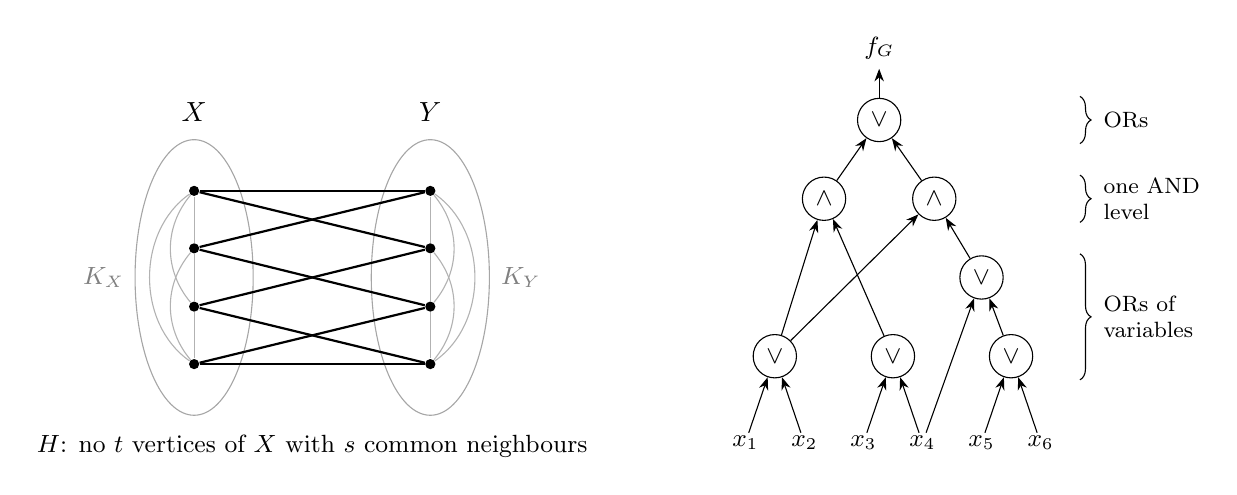
\begin{tikzpicture}[
  vtx/.style={circle,fill=black,inner sep=1.3pt},
  gate/.style={circle,draw,inner sep=0pt,minimum size=5.5mm,font=\small},
  inp/.style={font=\small,inner sep=1pt},
  wire/.style={-{Stealth[length=1.6mm]}},
  >=Stealth]
  % ---- left: the graph ----
  \draw[gray!70] (0,0) ellipse (0.75 and 1.75);
  \draw[gray!70] (3,0) ellipse (0.75 and 1.75);
  \node at (0,2.1) {$X$};
  \node at (3,2.1) {$Y$};
  \foreach \i/\y in {1/1.1,2/0.37,3/-0.37,4/-1.1} {
    \node[vtx] (x\i) at (0,\y) {};
    \node[vtx] (y\i) at (3,\y) {};
  }
  % cliques (drawn faintly)
  \foreach \pa/\pb in {1/2,2/3,3/4} {
    \draw[gray!60] (x\pa) -- (x\pb);
    \draw[gray!60] (y\pa) -- (y\pb);
  }
  \foreach \pa/\pb in {1/3,2/4} {
    \draw[gray!60] (x\pa) to[bend right=40] (x\pb);
    \draw[gray!60] (y\pa) to[bend left=40] (y\pb);
  }
  \draw[gray!60] (x1) to[bend right=55] (x4);
  \draw[gray!60] (y1) to[bend left=55] (y4);
  \node[gray,font=\small] at (-1.15,0) {$K_X$};
  \node[gray,font=\small] at (4.15,0) {$K_Y$};
  % bipartite part H
  \foreach \pa/\pb in {1/1,1/2,2/1,2/3,3/2,3/4,4/3,4/4} {
    \draw[thick] (x\pa) -- (y\pb);
  }
  \node[font=\small] at (1.5,-2.15) {$H$: no $t$ vertices of $X$ with $s$ common neighbours};

  % ---- right: a single-level circuit (fan-in two; operands of each AND have disjoint letters) ----
  \begin{scope}[xshift=7cm,yshift=-2.1cm]
    \foreach \i in {1,...,6} {
      \node[inp] (v\i) at ({(\i-1)*0.75},0) {$x_{\i}$};
    }
    \node[gate] (o1) at (0.375,1.1) {$\vee$};
    \node[gate] (o2) at (1.875,1.1) {$\vee$};
    \node[gate] (o3) at (3.375,1.1) {$\vee$};
    \node[gate] (o4) at (3.0,2.1) {$\vee$};
    \draw[wire] (v1) -- (o1); \draw[wire] (v2) -- (o1);
    \draw[wire] (v3) -- (o2); \draw[wire] (v4) -- (o2);
    \draw[wire] (v5) -- (o3); \draw[wire] (v6) -- (o3);
    \draw[wire] (o3) -- (o4); \draw[wire] (v4) -- (o4);
    \node[gate] (a1) at (1.0,3.1) {$\wedge$};
    \node[gate] (a2) at (2.4,3.1) {$\wedge$};
    \draw[wire] (o1) -- (a1); \draw[wire] (o2) -- (a1);
    \draw[wire] (o1) -- (a2); \draw[wire] (o4) -- (a2);
    \node[gate] (out) at (1.7,4.1) {$\vee$};
    \draw[wire] (a1) -- (out); \draw[wire] (a2) -- (out);
    \draw[wire] (out) -- ++(0,0.65) node[above,font=\small] {$f_G$};
    \draw[decorate,decoration={brace,amplitude=4pt}] (4.25,2.4) -- (4.25,0.8)
      node[midway,right=5pt,font=\footnotesize,align=left] {ORs of\\variables};
    \draw[decorate,decoration={brace,amplitude=4pt}] (4.25,3.4) -- (4.25,2.8)
      node[midway,right=5pt,font=\footnotesize,align=left] {one AND\\level};
    \draw[decorate,decoration={brace,amplitude=4pt}] (4.25,4.4) -- (4.25,3.8)
      node[midway,right=5pt,font=\footnotesize] {ORs};
  \end{scope}
\end{tikzpicture}

\end{adjustbox}
\caption{Left: $G=H\cup K_X\cup K_Y$; the bipartite part $H$ (thick) carries all the difficulty. Right: a single-level circuit computes ORs of variables, then one level of ANDs, then ORs.}\label{fig:setup}
\end{figure}

\section{The lower bound}

\begin{lemma}\label{lem:lower}
If $H$ is $(t,s)$-free then every single-level circuit for $f_G$ has at least $|E(H)|/(4(t-1)(s-1))$ gates.
\end{lemma}

For $t=s=2$ this is $|E(H)|\le 4\,\Cone(f_G)$. Up to the constant, the lemma is Lemma~3.13 of~\cite{Juk06}, which gives
$\Omega(|E(H)|/s^3)$ for $K_{s,s}$-free $H$; the argument below follows the Amano--Maruoka charging~\cite{AM06}.

\begin{proof}
Let $\Gamma$ be a single-level circuit computing $f_G$, with $|\Gamma|$ gates. Since there are no constants, every gate has a variable in its
cone; so if an AND gate $g$ reaches the output, every path from $g$ to the output consists of OR gates, both operands of
$g$ are AND-free, and $g(x)=1$ implies $f_G(x)=1$. Let $A,B$ be the letter sets of the operands of such a $g$. Then
$A\cap B=\emptyset$, since a common letter $z$ would give $f_G(e_z)=1$, and $A\times B\subseteq E(G)$, since $g=1$ on
$e_{x'}+e_{y'}$ for $x'\in A$, $y'\in B$. Hence $(A\cap X)\times(B\cap Y)\subseteq E(H)$, and $(t,s)$-freeness rules out
$|A\cap X|\ge t$ together with $|B\cap Y|\ge s$.

Fix an edge $uv$ of $H$, $u\in X$, $v\in Y$. On $e_u+e_v$ the output is $1$; descending from the output through OR gates
of value $1$ ends at a wire that is not an OR gate. It is not a variable, as $f_G$ vanishes on single vertices, so it is
an AND gate $g$ reaching the output with $g(e_u+e_v)=1$. Both operands of $g$ meet $\{u,v\}$ and they are disjoint, so
we may name them so that $u\in A$ and $v\in B$. Fix one such pair $(g,\text{naming})$ for each edge. Let $a=|A\cap X|$
and $b=|B\cap Y|$. We charge $uv$ to a code in $\{\text{gates}\}\times\{0,1\}\times\{0,1\}$:

\emph{Case $b\ge s$} (so $a\le t-1$; Figure~\ref{fig:charging}). In the AND-free cone of the operand with letters $B$, follow a path from the input
$x_v$ to that operand. The number of $Y$-letters is nondecreasing along it, starts at $1<s$ and ends at $b\ge s$. Let $h$
be the first wire with at least $s$ $Y$-letters; it is an OR gate, and its operand $o$ on the path contains $v$ and has
at most $s-1$ $Y$-letters. Charge $uv$ to $(h,\,\text{which operand of }h\text{ is }o,\,0)$.

\emph{Case $a\ge t$} (so $b\le s-1$). Symmetrically, walking from $x_u$ in the cone of the operand with letters $A$, let
$h$ be the first wire with at least $t$ $X$-letters and $o$ its operand on the path. Charge $uv$ to
$(h,\,\text{which operand},\,1)$.

\emph{Case $a\le t-1$, $b\le s-1$.} Charge $uv$ to $(g,\,\text{which operand of }g\text{ holds }u,\,0)$.

Codes of the first two cases have an OR gate in the first coordinate and are told apart by the last bit; codes of the
third case have an AND gate. Fix a code. In the first case $h$ is AND-free, so $S(h)$ and $S(o)$ depend only on the
code. Fix $s$ of the $Y$-letters of $h$ (depending only on $h$). Every edge $uv$ charged to the code has
$S(h)\cap Y\subseteq B\cap Y\subseteq N_H(u)$ for its own $g$, so $u$ is a common neighbour of these $s$ vertices: at
most $t-1$ choices. And $v\in S(o)\cap Y$: at most $s-1$ choices. The second case is symmetric ($t$ $X$-letters have at
most $s-1$ common neighbours; $u$ is one of fewer than $t$ $X$-letters of $o$). In the third case $u\in A\cap X$ and
$v\in B\cap Y$ with $A,B$ determined by the code: at most $ab\le(t-1)(s-1)$ edges. So every code receives at most
$(t-1)(s-1)$ edges, there are at most $4|\Gamma|$ codes, and $|E(H)|\le 4(t-1)(s-1)\,|\Gamma|$.
\end{proof}

\begin{figure}[t]
\centering
\begin{adjustbox}{max width=\linewidth}
% Figure 2: the charging step of Lemma 2, case b >= s.
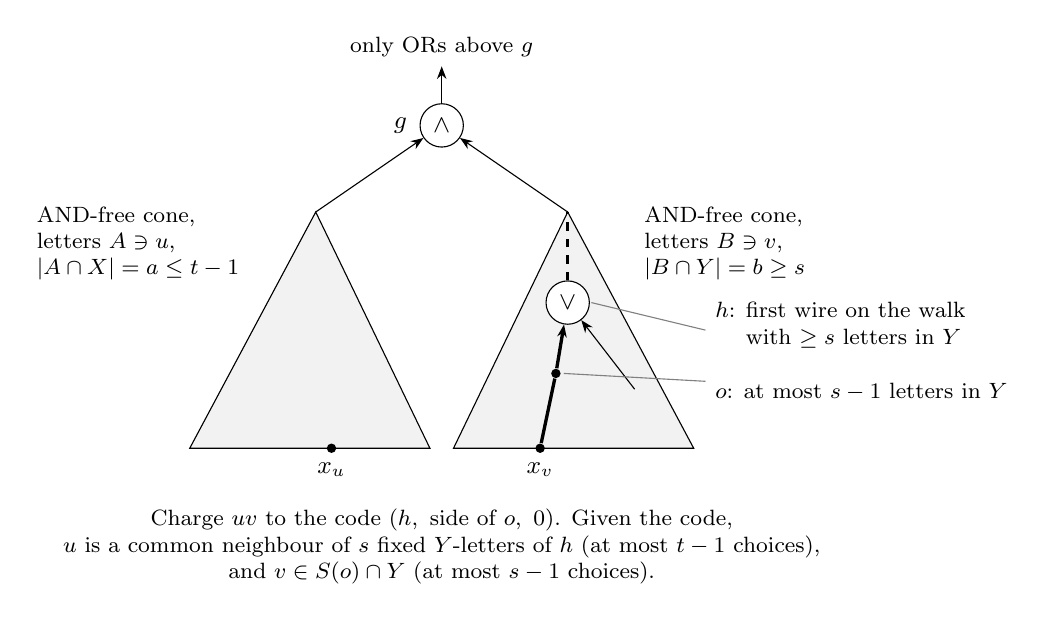
\begin{tikzpicture}[
  gate/.style={circle,draw,inner sep=0pt,minimum size=5.5mm,font=\small},
  pt/.style={circle,fill=black,inner sep=1.2pt},
  wire/.style={-{Stealth[length=1.6mm]}},
  note/.style={font=\footnotesize,align=left}]
  % the AND gate and its two AND-free operand cones
  \node[gate] (g) at (0,4.1) {$\wedge$};
  \node[left=1pt of g,font=\small] {$g$};
  \draw[wire] (g) -- ++(0,0.75) node[above,font=\footnotesize] {only ORs above $g$};
  \coordinate (aA) at (-1.6,3.0);
  \coordinate (aB) at (1.6,3.0);
  \fill[gray!10] (aA) -- (-3.2,0) -- (-0.15,0) -- cycle;
  \fill[gray!10] (aB) -- (0.15,0) -- (3.2,0) -- cycle;
  \draw (aA) -- (-3.2,0) -- (-0.15,0) -- cycle;
  \draw (aB) -- (0.15,0) -- (3.2,0) -- cycle;
  \draw[wire] (aA) -- (g);
  \draw[wire] (aB) -- (g);
  \node[note,anchor=east] at (-2.45,2.6) {AND-free cone,\\letters $A\ni u$,\\$|A\cap X|=a\le t-1$};
  \node[note,anchor=west] at (2.45,2.6) {AND-free cone,\\letters $B\ni v$,\\$|B\cap Y|=b\ge s$};
  % inputs
  \node[pt,label={below:{\small $x_u$}}] (xu) at (-1.4,0) {};
  \node[pt,label={below:{\small $x_v$}}] (xv) at (1.25,0) {};
  % walk from x_v to the operand
  \node[pt] (o) at (1.45,0.95) {};
  \node[gate,fill=white] (h) at (1.6,1.85) {$\vee$};
  \draw[very thick] (xv) -- (o);
  \draw[very thick,wire] (o) -- (h);
  \draw[very thick,dashed] (h) -- (aB);
  \draw[wire] (2.45,0.75) -- (h);
  \node[note,anchor=north west] at (3.35,0.95) {$o$: at most $s-1$ letters in $Y$};
  \node[note,anchor=south west] at (3.35,1.15) {$h$: first wire on the walk\\\phantom{$h$: }with $\ge s$ letters in $Y$};
  \draw[gray] (3.35,0.85) -- (1.55,0.95);
  \draw[gray] (3.35,1.5) -- (1.9,1.85);
  % the count
  \node[font=\footnotesize,align=center,anchor=north] at (0,-0.65) {%
    Charge $uv$ to the code $(h,\ \text{side of } o,\ 0)$. Given the code,\\
    $u$ is a common neighbour of $s$ fixed $Y$-letters of $h$ (at most $t-1$ choices),\\
    and $v\in S(o)\cap Y$ (at most $s-1$ choices).};
\end{tikzpicture}

\end{adjustbox}
\caption{Case $b\ge s$ in the proof of Lemma~\ref{lem:lower}. The walk from $x_v$ inside the AND-free cone of $g$'s second operand reaches a first wire $h$ with at least $s$ letters in $Y$; since $h$ is AND-free, the code $(h,\text{side},0)$ determines $S(h)$ and $S(o)$ whichever $g$ the edge used. The case $a\ge t$ is the mirror image with side bit~$1$.}\label{fig:charging}
\end{figure}

\section{The upper bound}

Let $X$ and $Y$ be identified with $\{0,1\}^m$ by an address map. For $j\le m$ and $e\in\{0,1\}$ let
$s^{e}_{X,j}=\bigvee\{x_u: u\in X,\ u_j=e\}$ and define $s^e_{Y,j}$ likewise. Let
$T_2(X)=\bigvee_j (s^0_{X,j}\wedge s^1_{X,j})$, which is $1$ iff at least two variables of $X$ are on.

\begin{lemma}[address-bit substitution, after~\cite{Juk06}]\label{lem:subst}
Let $\phi(\alpha,\beta)$ be a negation-normal-form circuit (resp.\ formula) over $\alpha,\beta\in\{0,1\}^m$ with
$\phi(\alpha,\beta)=1$ iff $\alpha\beta\in E(H)$. Replace each literal $\alpha_j$, $\neg\alpha_j$, $\beta_j$,
$\neg\beta_j$ by $s^1_{X,j}$, $s^0_{X,j}$, $s^1_{Y,j}$, $s^0_{Y,j}$ to get a monotone $\tilde\phi$. Then
\[ f_G = T_2(X)\vee T_2(Y)\vee\Big(\textstyle\bigvee_{X}x_u\wedge\bigvee_{Y}x_v\wedge\tilde\phi\Big). \]
Consequently $\Csize(f_G)\le 2mN+|\phi|+4m+O(1)$ with $N=2^m$, where $|\phi|$ is the number of gates of $\phi$, and
$f_G$ has a monotone formula with $\tfrac N2 L(\phi)+O(mN)$ leaves, where $L(\phi)$ is the leaf count of $\phi$.
\end{lemma}

\begin{proof}
If two variables on one side are on, they differ in some address bit, so $T_2=1=f_G$. If at most one is on per side and
one side is empty, then $T_2(X)=T_2(Y)=0$ and the guard $\bigvee_Xx_u\wedge\bigvee_Yx_v$ is $0$, as is $f_G$. If exactly
$u\in X$ and $v\in Y$ are on, each $s^e_{X,j}$ equals the truth value of $u_j=e$, so $\tilde\phi$ evaluates $\phi$ at
the addresses of $u$ and $v$. For the size (Figure~\ref{fig:upper}): the $4m$ sums take $N/2-1$ gates each, the guard reuses $s^0_{\cdot,1}\vee
s^1_{\cdot,1}$, and $T_2$ takes $2m-1$ gates per side.
\end{proof}

\begin{figure}[t]
\centering
\begin{adjustbox}{max width=\linewidth}
% Figure 3: the monotone circuit of Lemma 3 (address-bit substitution).
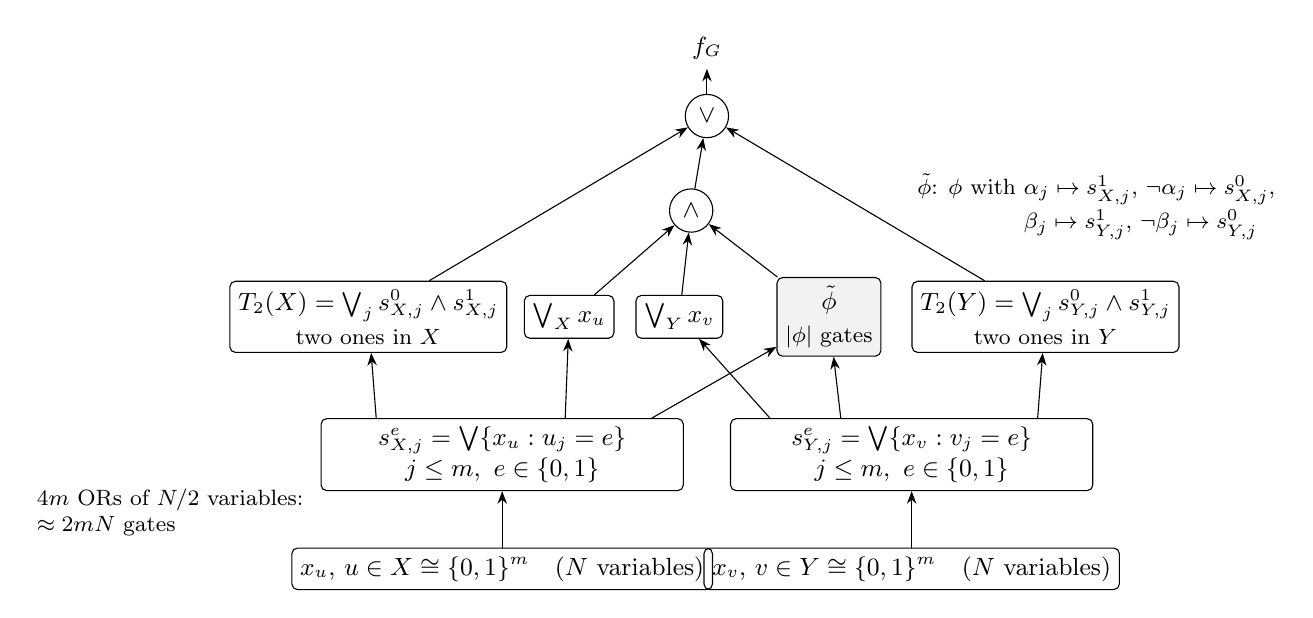
\begin{tikzpicture}[
  gate/.style={circle,draw,inner sep=0pt,minimum size=5.5mm,font=\small},
  blk/.style={draw,rounded corners=2pt,inner sep=3pt,font=\small,align=center},
  wire/.style={-{Stealth[length=1.6mm]}},
  note/.style={font=\footnotesize,align=left}]
  % variables
  \node[blk,minimum width=4.6cm] (VX) at (-2.6,0) {$x_u$,\ $u\in X\cong\{0,1\}^m$\quad($N$ variables)};
  \node[blk,minimum width=4.6cm] (VY) at (2.6,0) {$x_v$,\ $v\in Y\cong\{0,1\}^m$\quad($N$ variables)};
  % address sums
  \node[blk,minimum width=4.6cm] (SX) at (-2.6,1.45) {$s^{e}_{X,j}=\bigvee\{x_u : u_j=e\}$\\ $j\le m,\ e\in\{0,1\}$};
  \node[blk,minimum width=4.6cm] (SY) at (2.6,1.45) {$s^{e}_{Y,j}=\bigvee\{x_v : v_j=e\}$\\ $j\le m,\ e\in\{0,1\}$};
  \draw[wire] (VX) -- (SX);
  \draw[wire] (VY) -- (SY);
  \node[note,anchor=east] at (-5.0,0.72) {$4m$ ORs of $N/2$ variables:\\$\approx 2mN$ gates};
  % middle layer
  \node[blk] (T2X) at (-4.3,3.2) {$T_2(X)=\bigvee_j s^0_{X,j}\wedge s^1_{X,j}$\\[1pt]{\footnotesize two ones in $X$}};
  \node[blk] (T2Y) at (4.3,3.2) {$T_2(Y)=\bigvee_j s^0_{Y,j}\wedge s^1_{Y,j}$\\[1pt]{\footnotesize two ones in $Y$}};
  \node[blk] (GX) at (-1.75,3.2) {$\bigvee_X x_u$};
  \node[blk] (GY) at (-0.35,3.2) {$\bigvee_Y x_v$};
  \node[blk,fill=gray!10] (phi) at (1.55,3.2) {$\tilde\phi$\\[1pt]{\footnotesize $|\phi|$ gates}};
  \draw[wire] (SX.north) ++(-1.6,0) -- (T2X);
  \draw[wire] (SY.north) ++(1.6,0) -- (T2Y);
  \draw[wire] (SX.north) ++(0.8,0) -- (GX);
  \draw[wire] (SY.north) ++(-1.8,0) -- (GY);
  \draw[wire] (SX.north) ++(1.9,0) -- (phi);
  \draw[wire] (SY.north) ++(-0.9,0) -- (phi);
  \node[gate] (and) at (-0.2,4.55) {$\wedge$};
  \draw[wire] (GX) -- (and); \draw[wire] (GY) -- (and); \draw[wire] (phi) -- (and);
  \node[gate] (out) at (0,5.75) {$\vee$};
  \draw[wire] (T2X) -- (out); \draw[wire] (and) -- (out); \draw[wire] (T2Y) -- (out);
  \draw[wire] (out) -- ++(0,0.6) node[above,font=\small] {$f_G$};
  % substitution rule
  \node[note,anchor=west] at (2.55,4.6) {$\tilde\phi$: $\phi$ with $\alpha_j\mapsto s^1_{X,j}$,\ $\neg\alpha_j\mapsto s^0_{X,j}$,\\
    \phantom{$\tilde\phi$: $\phi$ with }$\beta_j\mapsto s^1_{Y,j}$,\ $\neg\beta_j\mapsto s^0_{Y,j}$};
\end{tikzpicture}

\end{adjustbox}
\caption{The monotone circuit of Lemma~\ref{lem:subst}. The $4m$ address sums dominate the size; the adjacency test enters only through $\tilde\phi$, whose size is that of the non-monotone circuit $\phi$.}\label{fig:upper}
\end{figure}

\subsection{Norm graphs}

Let $q=2^k$, $F=\GF(q^t)$, $m=kt$, $N=q^t$, and $\Nm(z)=z^{1+q+\dots+q^{t-1}}$. The bipartite norm graph $H$ has
$X=Y=F$ and $x\sim y$ iff $\Nm(x+y)=1$. Each vertex has degree $(q^t-1)/(q-1)$, so $|E(H)|\ge N^{2-1/t}$, and by
Koll\'ar, R\'onyai and Szab\'o~\cite{KRS96} any $t$ distinct $x_1,\dots,x_t$ have at most $t!$ common neighbours; since
$H$ is symmetric, $H$ is $(t,t!+1)$-free. (We use the statement as given in~\cite[Example~13.24]{BFC}.
TODO: compare with~\cite{KRS96} directly.)

\begin{lemma}\label{lem:normcircuit}
``$\Nm(\alpha+\beta)=1$'' has a negation-normal-form circuit with $O(tm^2)$ gates and formula with $m^{O(\log t)}$
leaves.
\end{lemma}

\begin{proof}
Fix a basis of $F$ over $\GF(2)$. Addition is coordinatewise XOR; each Frobenius power $z\mapsto z^{q^i}$ is
$\GF(2)$-linear, so each output coordinate is an XOR of at most $m$ input coordinates; multiplication is
$\GF(2)$-bilinear, so each output coordinate is an XOR of at most $m^2$ products of coordinates. Compute the $t$
conjugates of $z=\alpha+\beta$, multiply them in a balanced binary tree of depth $\lceil\log_2 t\rceil$, and test the
result against the coordinates of $1$ with an AND of $m$ literals. In dual-rail form an XOR costs $O(1)$ gates, giving
$O(tm^2)$ gates. For formulas, a balanced XOR of $R$ dual-rail formulas has $O(R^2)$ times their leaves, so each level
of the product tree multiplies leaf counts by $O(m^4)$, and the total is $m\cdot O(m^2)\cdot O(m^4)^{\lceil\log_2
t\rceil}=m^{O(\log t)}$.
\end{proof}

\begin{remark}
Explicitness requires a representation of $\GF(2^m)$; an irreducible polynomial of degree $m$ over $\GF(2)$ can be
found deterministically in time polynomial in $m$. TODO [unchecked]: cite Shoup (1990), as suggested by a reviewer.
\end{remark}

\begin{proof}[Proof of Theorem~\ref{thm:main}]
Take $H$ the norm graph and $n=2N$. Lemma~\ref{lem:lower} with $s=t!+1$ gives $\Cone(f_G)\ge
N^{2-1/t}/(4(t-1)t!)$. Lemmas~\ref{lem:subst} and~\ref{lem:normcircuit} give $\Csize(f_G)\le 2mN+O(tm^2)=(1+o(1))\,n
\log_2 n$ for fixed $t$ as $k\to\infty$, and formulas with $N m^{O(\log t)}$ leaves.
\end{proof}

\section{The case \texorpdfstring{$t=2$}{t=2} in Lean}\label{sec:lean}

Let $F=\GF(2^k)$, $X=Y=F^2$, and $(a,b)\sim(c,d)$ iff $ac=b+d$: the sum-product graph~\cite[Example~7.5]{BFC}. It has
$N^{3/2}$ edges ($N=4^k$) and no 4-cycle, since two equations $ax=b+y$, $cx=d+y$ with $(a,b)\ne(c,d)$ have at most one
common solution. Adjacency is a test of $2k$ coordinate equations, each a bilinear form plus a linear form.

The Lean development (Lean~4.36, Mathlib; project \texttt{single-level-gap} of \url{https://github.com/prasincs/formal-math})
defines circuits, single-level circuits and monotone formulas from scratch and proves, for every $k\ge 1$:
\begin{itemize}
\item every single-level circuit with $M$ gates computing $f_G$ satisfies $8^k\le 4M$ (that is,
$|E(H)|\le 4\,\Cone(f_G)$; the general lemma \texttt{single\_level\_lower} holds for every 4-cycle-free bipartite $H$);
\item $f_G$ has a monotone formula with at most $4^k\,(8k+2+8k(k^2+2)^2)$ leaves.
\end{itemize}
The theorems depend only on the axioms \texttt{propext}, \texttt{Classical.choice} and \texttt{Quot.sound}, and a second,
independent kernel (nanoda) accepts the exported proofs and rejects ten tampered copies that change what is claimed. This gives an explicit gap of
$\sqrt N/O(k^5)=n^{1/2-o(1)}$ against formulas. TODO: decide whether to formalize Lemma~\ref{lem:lower} for general
$(t,s)$; the norm-graph freeness theorem is not in Mathlib.

\section{Remarks}

\begin{figure}[t]
\centering
% Figure 4: computed gap for norm graphs. Data: normgap dat t 64 (see figures/README.md).
% Colours: categorical slots 1-3 of the default dataviz palette; marks and direct labels carry identity too.
\definecolor{seriesA}{HTML}{2A78D6}
\definecolor{seriesB}{HTML}{EB6834}
\definecolor{seriesC}{HTML}{1BAF7A}
\begin{tikzpicture}
  \begin{axis}[
    width=0.82\textwidth, height=0.5\textwidth,
    xmin=0, xmax=72, ymin=-10, ymax=36,
    xlabel={$\log_2 n$},
    ylabel={$\log_2\bigl(\text{lower bound on } C_1(f_G)\,/\,\text{upper bound on } C(f_G)\bigr)$},
    ylabel style={font=\footnotesize},
    xlabel style={font=\small},
    tick label style={font=\footnotesize},
    xtick={0,8,...,64}, ytick={-8,0,8,...,32},
    axis lines=left,
    grid=major, grid style={gray!20, line width=0.3pt},
    legend style={font=\footnotesize, draw=none, fill=white, at={(0.03,0.97)}, anchor=north west},
    legend cell align=left,
    clip=false,
  ]
    \addplot[gray, line width=0.6pt, dashed, forget plot] coordinates {(0,0) (66,0)};
    \node[font=\scriptsize, gray, anchor=south east] at (axis cs:66,0) {gap $=1$};
    \addplot[seriesA, line width=1pt, mark=*, mark size=1.4pt]
      table[x=logn, y=gapcirc] {figures/gap-t2.dat};
    \addlegendentry{$t=2$, $C_1/C\ge n^{1/2-o(1)}$}
    \addplot[seriesB, line width=1pt, mark=square*, mark size=1.4pt]
      table[x=logn, y=gapcirc] {figures/gap-t3.dat};
    \addlegendentry{$t=3$, $C_1/C\ge n^{2/3-o(1)}$}
    \addplot[seriesC, line width=1pt, mark=triangle*, mark size=1.8pt]
      table[x=logn, y=gapcirc] {figures/gap-t4.dat};
    \addlegendentry{$t=4$, $C_1/C\ge n^{3/4-o(1)}$}
    \node[font=\footnotesize, anchor=west] at (axis cs:65.6,22.0) {$t=2$};
    \node[font=\footnotesize, anchor=west] at (axis cs:64.6,29.44) {$t=3$};
    \node[font=\footnotesize, anchor=west] at (axis cs:65.6,32.83) {$t=4$};
  \end{axis}
\end{tikzpicture}

\caption{The proven gap bound for norm graphs: $\log_2$ of the lower bound of Lemma~\ref{lem:lower} on $\Cone(f_G)$ divided by the size of the circuit of Lemma~\ref{lem:subst}, for $q=2^k$ and $n=2q^t\le 2^{65}$. The slopes approach $1-1/t$; the gap exceeds $1$ above the dashed line. The true gap can only be larger.}\label{fig:gap}
\end{figure}

\begin{itemize}
\item The constant factors are large. With the circuit bound, the computed gap for norm graphs exceeds $1$ only
from about $n\approx 2^{17}$ ($t=2,3$) or $2^{19}$ ($t=4$); against formulas, only at astronomically large $n$.
Figure~\ref{fig:gap} plots these values. They were computed by our program, which builds $\phi$ gate by gate
over a fixed irreducible polynomial, counts the circuit of Lemma~\ref{lem:subst} exactly, and uses the lower bound
$|E(H)|/(4(t-1)\,t!)$; $\phi$ was checked against direct field arithmetic on all input pairs for
$(k,t)\in\{(1,2),(2,2),(3,2),(4,2),(1,3),(2,3),(1,4)\}$.
\item Theorem~\ref{thm:main} does not give a linear gap: the counting argument of~\cite{Juk06} gives
$n/\log^{O(1)}n$ for non-explicit graphs. Is there an explicit graph with $\Cone(f_G)/\Csize(f_G)=n^{1-o(1)}$?
Projective norm graphs~\cite{ARS99} [unchecked] improve $t!$ to $(t-1)!$ but not the exponent.
\end{itemize}

\paragraph{Acknowledgements.} Much of this work was done with AI assistants; Appendix~\ref{app:ai} describes
what they did and how their output was checked.

\appendix
\section{Use of AI tools}\label{app:ai}

AI systems are not authors of this paper; the author takes responsibility for all of its content. Because their
part was substantial, we describe it so that readers can weigh the results accordingly.

\paragraph{Claude (Anthropic).} The work was carried out with Claude agents, run as a group with separate roles,
under the author's direction. They searched the literature, found Problem~22 in the original ECCC version
of~\cite{JukTR}, and checked whether the explicit gap was already known. They proposed the sum-product graph for
$t=2$ and its generalization to norm graphs, wrote the proofs of Lemmas~\ref{lem:lower}--\ref{lem:normcircuit} in
their present form, and wrote the Lean development of Section~\ref{sec:lean}. They also wrote the program behind
Figure~\ref{fig:gap} and the figures, and drafted the text.

\paragraph{Gemini (Google).} Two Gemini models, from a different model family, refereed Lemma~\ref{lem:lower},
Lemma~\ref{lem:subst} and the gap estimate independently. One of them found that an earlier version of the charging
argument did not separate the two walk cases, and gave a six-vertex instance where two edges received the same code;
the side bit in the proof of Lemma~\ref{lem:lower} fixes this. The reviews also led to the asymptotic form of
Theorem~\ref{thm:main} and to the remark on constructing $\GF(2^m)$.

\paragraph{How the output was checked.} The statements of Section~\ref{sec:lean} are checked by the Lean kernel and by nanoda, an independent kernel.
The adjacency circuit used in Figure~\ref{fig:gap} was checked against direct field arithmetic on all inputs for small
fields. All other arguments were checked by the author and by the reviews above, not by machine. Citations marked
[unchecked] have not yet been compared with the sources.

\paragraph{The author's part.} The author chose the line of work, directed and reviewed the agents, decided what to
pursue and what to claim, and checked the arguments.
% TODO (author): confirm that this paragraph describes your part accurately, and add anything missing.


\begin{thebibliography}{9}
\bibitem{AM06} K.~Amano and A.~Maruoka. On the monotone circuit complexity of quadratic Boolean functions.
\emph{Algorithmica} 46 (2006) 3--14. Preliminary version in ISAAC 2004, LNCS 3341, 28--40.
\bibitem{Juk06} S.~Jukna. Disproving the single level conjecture. \emph{SIAM J. Comput.} 36(1) (2006).
TODO: page numbers.
\bibitem{JukTR} S.~Jukna. Disproving the single level conjecture. ECCC TR05-021, original version (February 2005),
Problem~22.
\bibitem{BFC} S.~Jukna. \emph{Boolean Function Complexity: Advances and Frontiers}. Springer, 2012.
\bibitem{KRS96} J.~Koll\'ar, L.~R\'onyai and T.~Szab\'o. Norm-graphs and bipartite Tur\'an numbers.
\emph{Combinatorica} 16 (1996). TODO [unchecked]: pages; compare statement.
\bibitem{ARS99} N.~Alon, L.~R\'onyai and T.~Szab\'o. Norm-graphs: variations and applications.
\emph{J. Combin. Theory Ser. B} 76 (1999). TODO [unchecked].
\end{thebibliography}
\end{document}
